\documentclass[11pt]{article}

\usepackage[margin=1in]{geometry}
\usepackage{amsmath,amssymb}
\usepackage[T1]{fontenc}
\usepackage[utf8]{inputenc}
\usepackage{lmodern}
\usepackage{microtype}
\usepackage{booktabs}
\usepackage{graphicx}
\usepackage{enumitem}
\usepackage{caption}
\usepackage{xcolor}
\usepackage[hidelinks]{hyperref}

\captionsetup{font=small,labelfont=bf}
\setlist{nosep,leftmargin=1.4em}
\definecolor{teal}{HTML}{0E8F82}

\newcommand{\mxF}[1]{\textbf{#1}}

\title{\LARGE\bfseries Encrypted Real-Time Communication Application\\[2pt] Identification from Five Packet Measurements}
\author{\large Siddhant Parashar\\[2pt] \normalsize CyberAI Cup 2026 --- Task 3}
\date{}

\begin{document}

\maketitle

\begin{abstract}
\noindent
Real-time communication (RTC) applications such as Discord, Google Meet, Messenger, WhatsApp and Zoom
encrypt their media end-to-end with SRTP over DTLS, so payload inspection is unavailable. This work
addresses the resulting identification problem: given only the \emph{sizes and inter-arrival times of the
first five packets} of an encrypted UDP media flow, predict the originating application and whether the
call is voice or video---a ten-class problem. We contribute (i) a domain-grounded feature set of 241
deterministic descriptors derived from the encrypted-traffic-analysis literature; (ii) a leakage-aware
grouped cross-validation protocol that accounts for the unpublished call identifiers in the dataset;
(iii) a systematic three-round experimental campaign spanning 2{,}377 hyperparameter points, a
self-supervised transformer pretrained on 90{,}610 auxiliary flows, tabular foundation models, and a set
of customized linear probes; and (iv) a precise characterisation of the dataset's \emph{label geometry},
which shows that 160 of 1{,}285 training flows are provably unclassifiable because a video call whose first
five packets contain no video fragment is physically indistinguishable from a voice call. The final
architecture---a flat ten-class head averaged with a hierarchical application$\times$mode composition,
over a TabICL tabular foundation model, followed by one parameter-free decision rule---achieves
\mxF{84.22\% accuracy and 82.92\% macro-F1 under grouped cross-validation}, against a measured ceiling of
93.77\% accuracy and 93.64\% macro-F1. We report all ablations, including the negative ones, and show that
the residual error is concentrated in the irreducibly ambiguous Zoom voice/video pair.

\medskip
\noindent\textbf{Keywords:} encrypted traffic classification; real-time communication; packet-length
fingerprinting; tabular foundation models; grouped cross-validation; linear probes; self-supervised
pretraining.
\end{abstract}

\tableofcontents
\newpage

%==================================================================
\section{Introduction}
%==================================================================

Real-time communication applications carry a substantial and growing fraction of interactive Internet
traffic. Their media streams are protected end-to-end by SRTP over DTLS, which provides confidentiality,
integrity and replay protection but also removes every avenue of deep-packet inspection. Identifying which
application generated a flow---and whether a call is audio-only or audio-plus-video---must therefore
proceed from \emph{behavioural side-channels}: most notably the sizes and timings of encrypted packets.

The competition task formalises this as a ten-class classification problem over the cross product of five
applications (Discord, Google Meet, Messenger, WhatsApp, Zoom) and two call modes (voice, video). The input
for each flow is deliberately minimal: five packets, described by their cumulative arrival time and UDP
payload length. The training set holds 1{,}285 labelled flows; the held-out test set holds 327.

This paper reports the full lifecycle of our solution. Three contributions stand out.

\begin{enumerate}
\item \textbf{A leakage-aware evaluation protocol.} The training flows are drawn from 400 source calls
while the test flows come from 100 \emph{held-out} calls, but no call identifier is published. Multiple
flows from one call are near-identical, so a naive random split scores a memorised call rather than a
generalising model. We introduce a pseudo-group key and evaluate everything under \emph{grouped}
cross-validation, which we argue is the only honest estimate available.
\item \textbf{A measured characterisation of the task's ceiling.} We show that the dataset contains an
exactly balanced, inseparable subset: 160 Zoom flows whose five-packet windows are audio-only, 80 of which
are voice and 80 video, at coin-flip discriminability (grouped-CV AUC 0.55). This caps the entire task at
93.77\% accuracy and 93.64\% macro-F1, and it licenses one \emph{parameter-free} decision rule that every
model family we tested benefits from.
\item \textbf{A large, fully-reported ablation campaign.} Across three rounds we score 2{,}377
hyperparameter points, train a self-supervised transformer on a 6.97\,GB auxiliary corpus, evaluate two
tabular foundation models, build five linear probes, and test call-structure recovery---and we report the
negative results with the same care as the positive ones, because they are what prevent a reader from
repeating the same dead ends.
\end{enumerate}

%==================================================================
\section{Related Work}
%==================================================================

Encrypted traffic classification rests on two observations. First, the codec and transport stack leaves a
fingerprint in the \emph{statistical distribution} of packet sizes: Taylor et al.'s \emph{AppScanner} built
classifiers from packet-size summaries; Draper-Gil et al.'s \emph{ISCXVPN} added time-based flow features.
Second, the \emph{sequence} of sizes and inter-arrival gaps carries further structure: Korczy\'nski \& Duda
used first-order Markov chains over quantised sizes; Shapira \& Shavitt's \emph{FlowPic} treated the
size--time plane as an image; Lopez-Martin et al.\ applied CNNs and RNNs directly to per-packet sequences.

Three strands from 2024--2025 are directly relevant to our later decisions. \textbf{Tabular foundation
models} prior-fitted on synthetic datasets---TabPFN and its successors, TabICL---report state-of-the-art
performance on datasets below 10{,}000 rows with no task-specific training, which is precisely our regime.
\textbf{Traffic-specific pretrained transformers} (ET-BERT, YaTC, TrafficFormer, FlowletFormer) extend
masked-modelling to packet streams. \textbf{Passive RTC measurement} (Michel et al.'s IMC'22 analysis of
Zoom; recent work on encrypted video QoE) shows that even without payload, per-application header stacks and
size families leak media type. Finally, the \textbf{MIRAGE} corpus from the University of Naples, and the
MIMETIC/DISTILLER line of work built on it, supplies labelled mobile-application captures that we use as an
auxiliary pretraining and probe source.

Our evaluation protocol additionally engages with a methodological problem specific to traffic data: the
\emph{correlated-flows} property---several flows from one session---which, if ignored, inflates validation
scores. Semi-supervised and clustering methods that exploit this property (X-Means with label propagation,
SemTra) motivate one of our ablation branches.

%==================================================================
\section{Dataset and Problem Formulation}
%==================================================================

\subsection{Data format}

Each row is one media flow described by its first five packets, interleaved as
$(\texttt{relative\_time}_i, \texttt{packet\_length}_i)$ for $i \in \{0,\dots,4\}$.
\texttt{relative\_time\_0} is identically zero; times are cumulative with microsecond precision; lengths
are UDP payload sizes (total length minus the 8-byte UDP header). The target is one of ten case-sensitive
strings encoding \texttt{application\_mode}.

\begin{table}[htbp]
\centering\small
\caption{Dataset summary.}
\label{tab:data}
\begin{tabular}{lc}
\toprule
Property & Value \\
\midrule
Training flows / test flows & 1{,}285 / 327 \\
Columns per flow & 10 + label \\
Packet length range & 26--1{,}242 bytes \\
Five-packet time span & 48\,\textmu s--23.2\,s (median 571\,\textmu s) \\
Class imbalance & 6.4$\times$ (Discord\_video 256 $\rightarrow$ GoogleMeet\_voice 40) \\
Missing values / reordered timestamps & none \\
\bottomrule
\end{tabular}
\end{table}

\subsection{Integrity and leakage structure}

Exploratory analysis established three facts that shaped everything downstream.

\begin{enumerate}
\item \textbf{The label is almost determined by the length tuple.} 1{,}136 distinct length tuples exist;
only \textbf{2} map to more than one class, covering 95 rows (7.4\%)---the repeated constant-size keepalive
patterns. The Bayes floor is therefore near zero \emph{outside} those tuples; the difficulty is
generalisation, not label noise.
\item \textbf{Train and test are exchangeable.} A train-vs-test discriminator scores \textbf{AUC 0.529},
essentially chance, so cross-validation is a meaningful proxy for the leaderboard.
\item \textbf{Group structure is real but moderate.} 1{,}107 pseudo-groups; 253 flows (20\%) share a
near-duplicate signature with another flow. Because the test split is drawn from held-out calls, a plain
stratified split leaks.
\end{enumerate}

\begin{figure}[htbp]
\centering
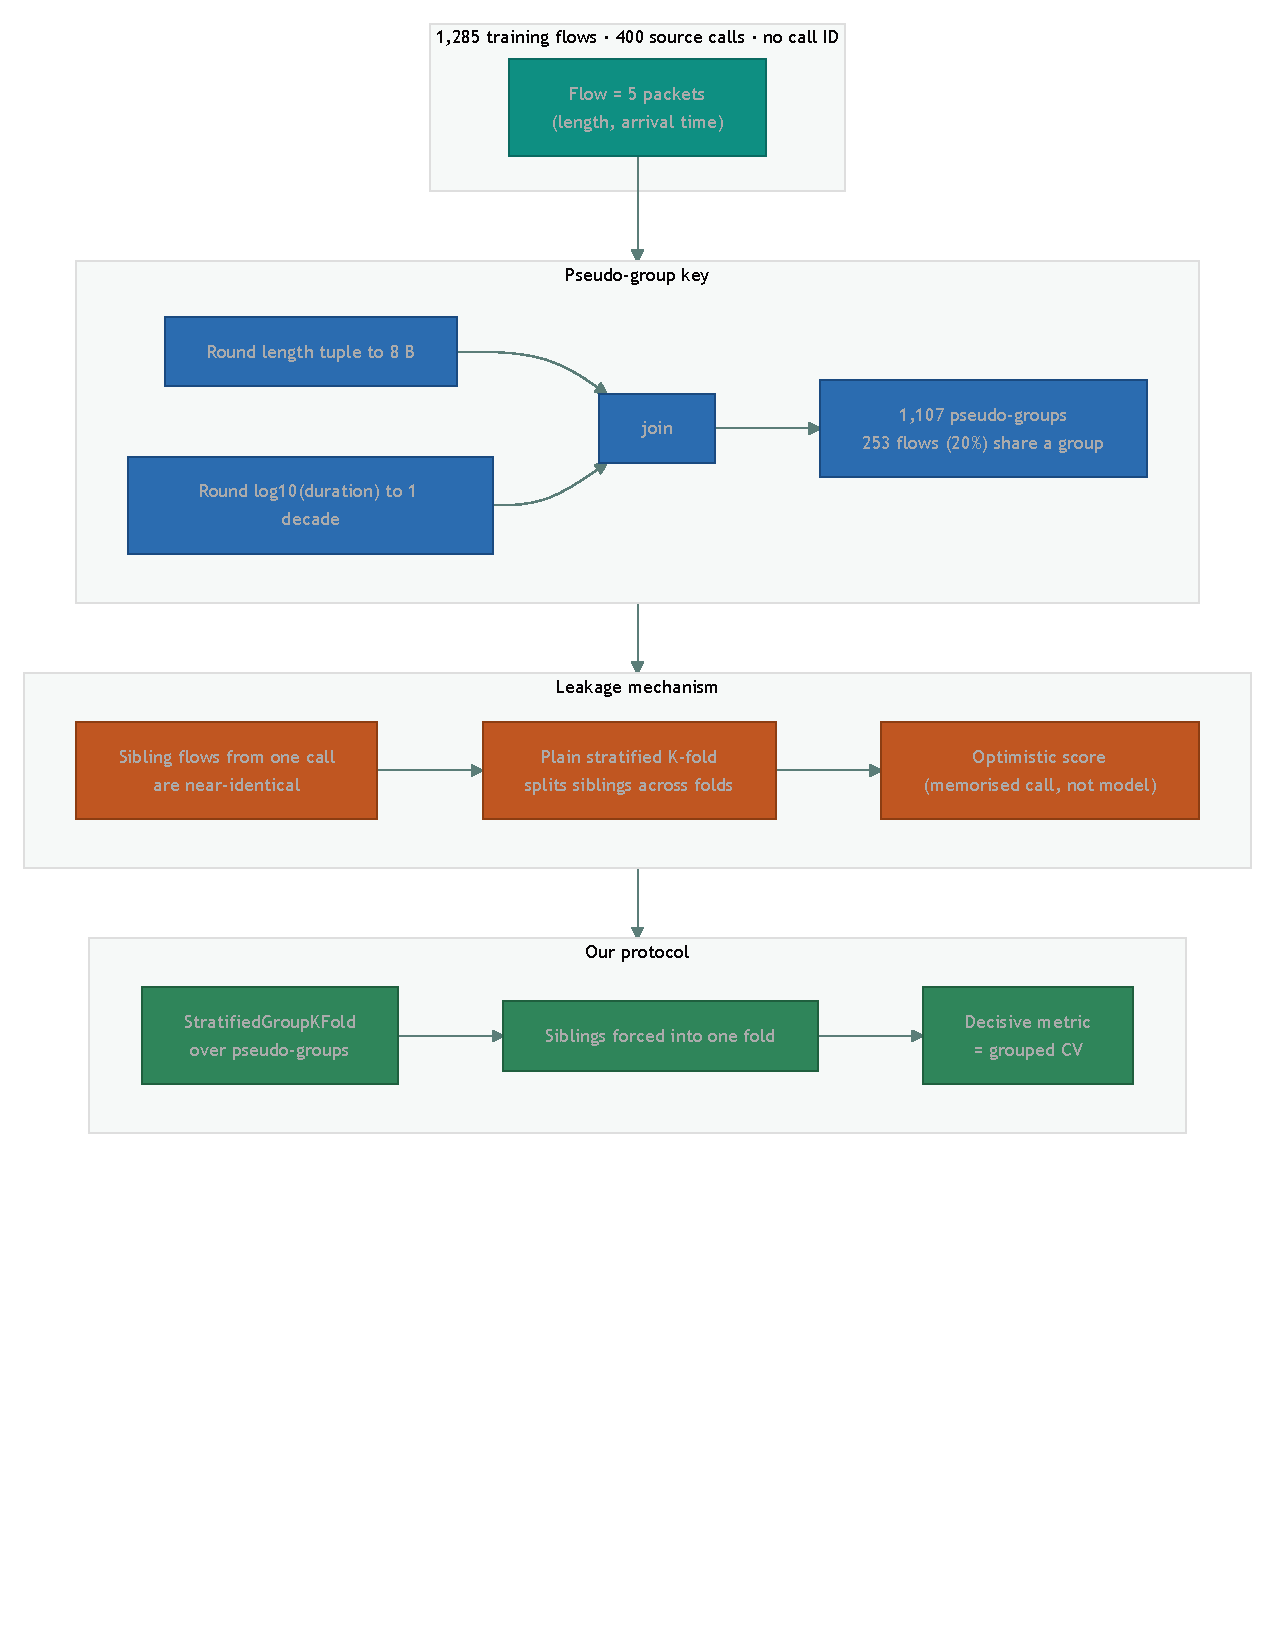
\includegraphics[width=\textwidth]{figures/diagram_1.pdf}
\caption{The leakage mechanism introduced by unpublished call identifiers, and the grouped
cross-validation protocol we adopt in response.}
\label{fig:leakage}
\end{figure}

\subsection{Evaluation protocol}

Every model is scored under \textbf{two} schemes in parallel.

\begin{itemize}
\item \textbf{\texttt{plain}} --- \texttt{RepeatedStratifiedKFold} (5 folds, 3 repeats, seed 42). The
optimistic estimate, retained for comparability with published baselines.
\item \textbf{\texttt{group}} --- \texttt{StratifiedGroupKFold} (5 folds) over the pseudo-group key,
repeated twice with different shuffles. \textbf{This is the decisive number} and every selection decision
in this paper uses it.
\end{itemize}

Fold indices are computed once and stored, so scores from different runs and containers are directly
comparable. The primary metric is accuracy (implied by the submission format); macro-F1 and macro-recall
are tracked as secondary metrics because the test distribution is explicitly not guaranteed uniform.

%==================================================================
\section{Methodology}
%==================================================================

\subsection{System overview}

\begin{figure}[htbp]
\centering
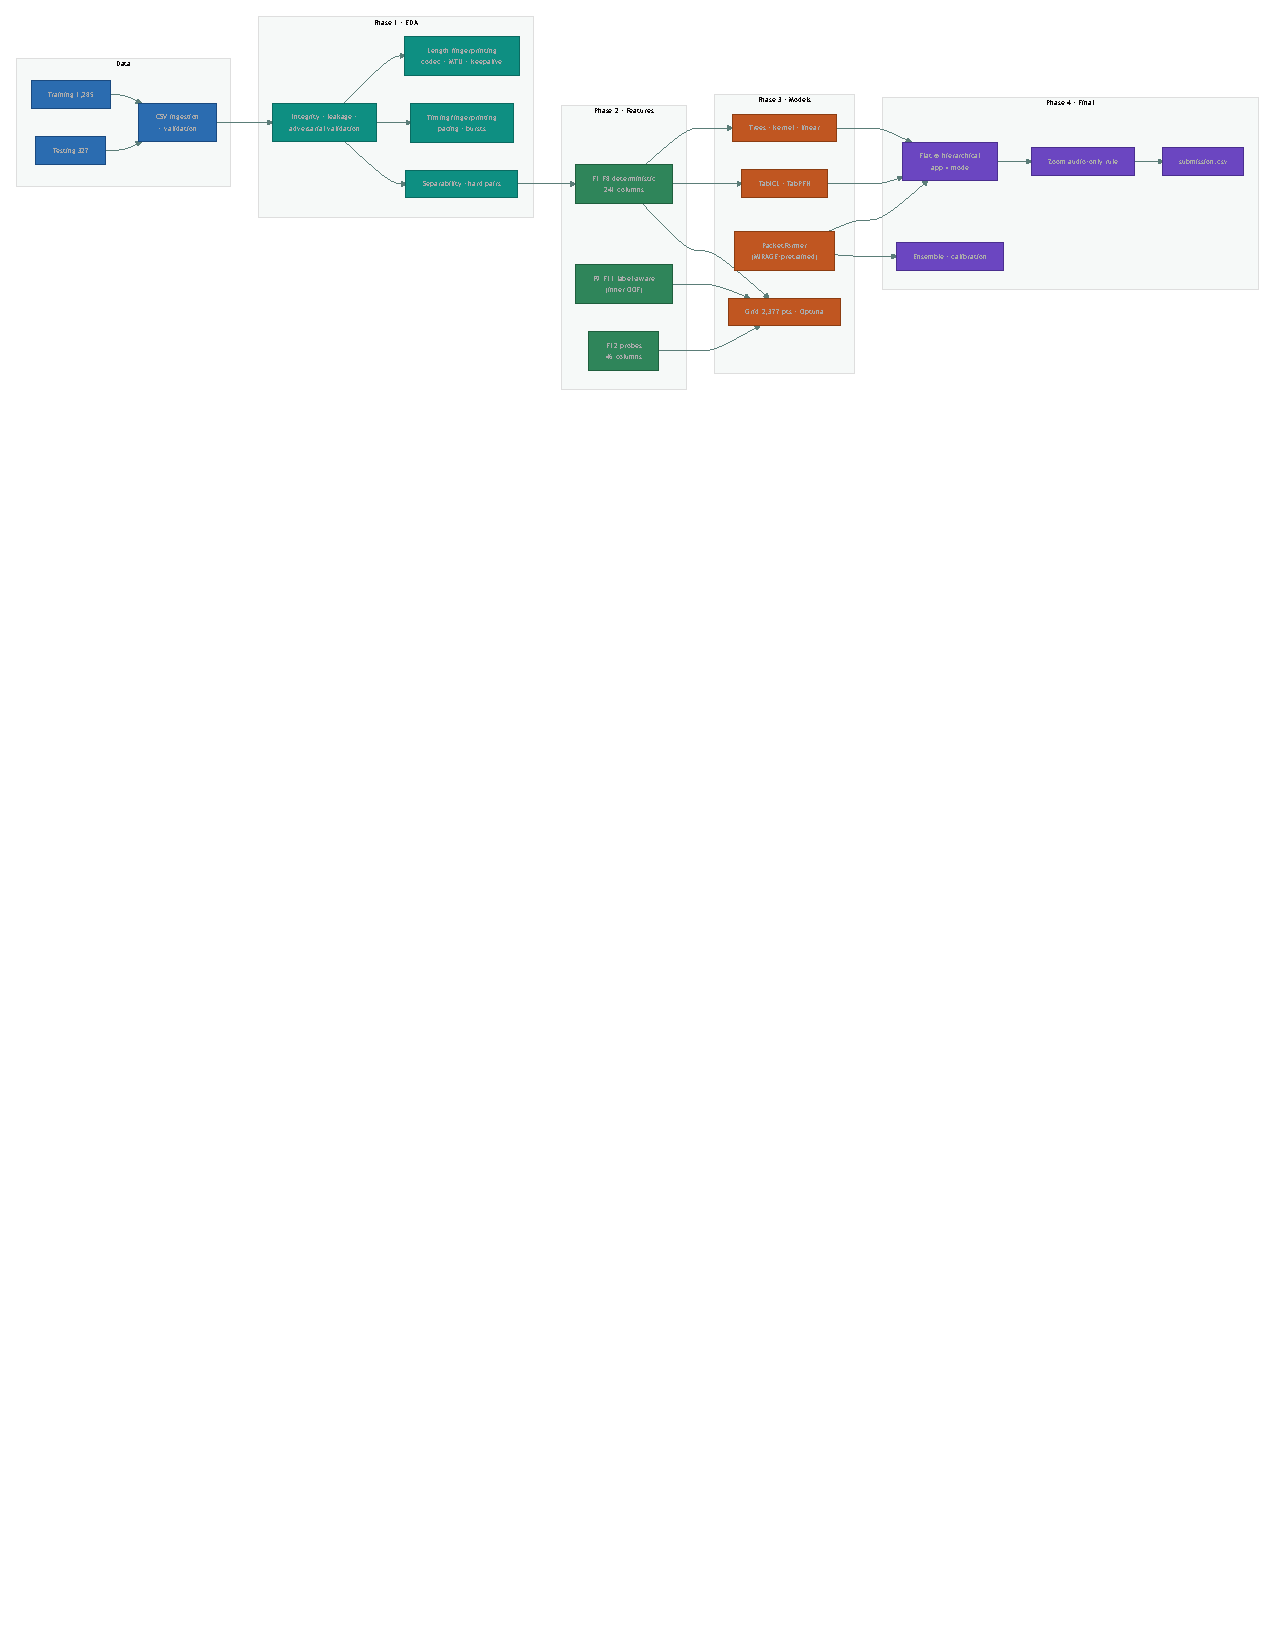
\includegraphics[width=\textwidth]{figures/diagram_2.pdf}
\caption{End-to-end pipeline, from ingestion through the four phases to the final submission.}
\label{fig:overview}
\end{figure}

\subsection{Feature engineering}

We engineer twelve feature blocks grounded in the encrypted-traffic literature. The decisive design choice
is the split between \emph{deterministic} blocks and \emph{fitted} blocks (Figure~\ref{fig:features}).

\begin{figure}[htbp]
\centering
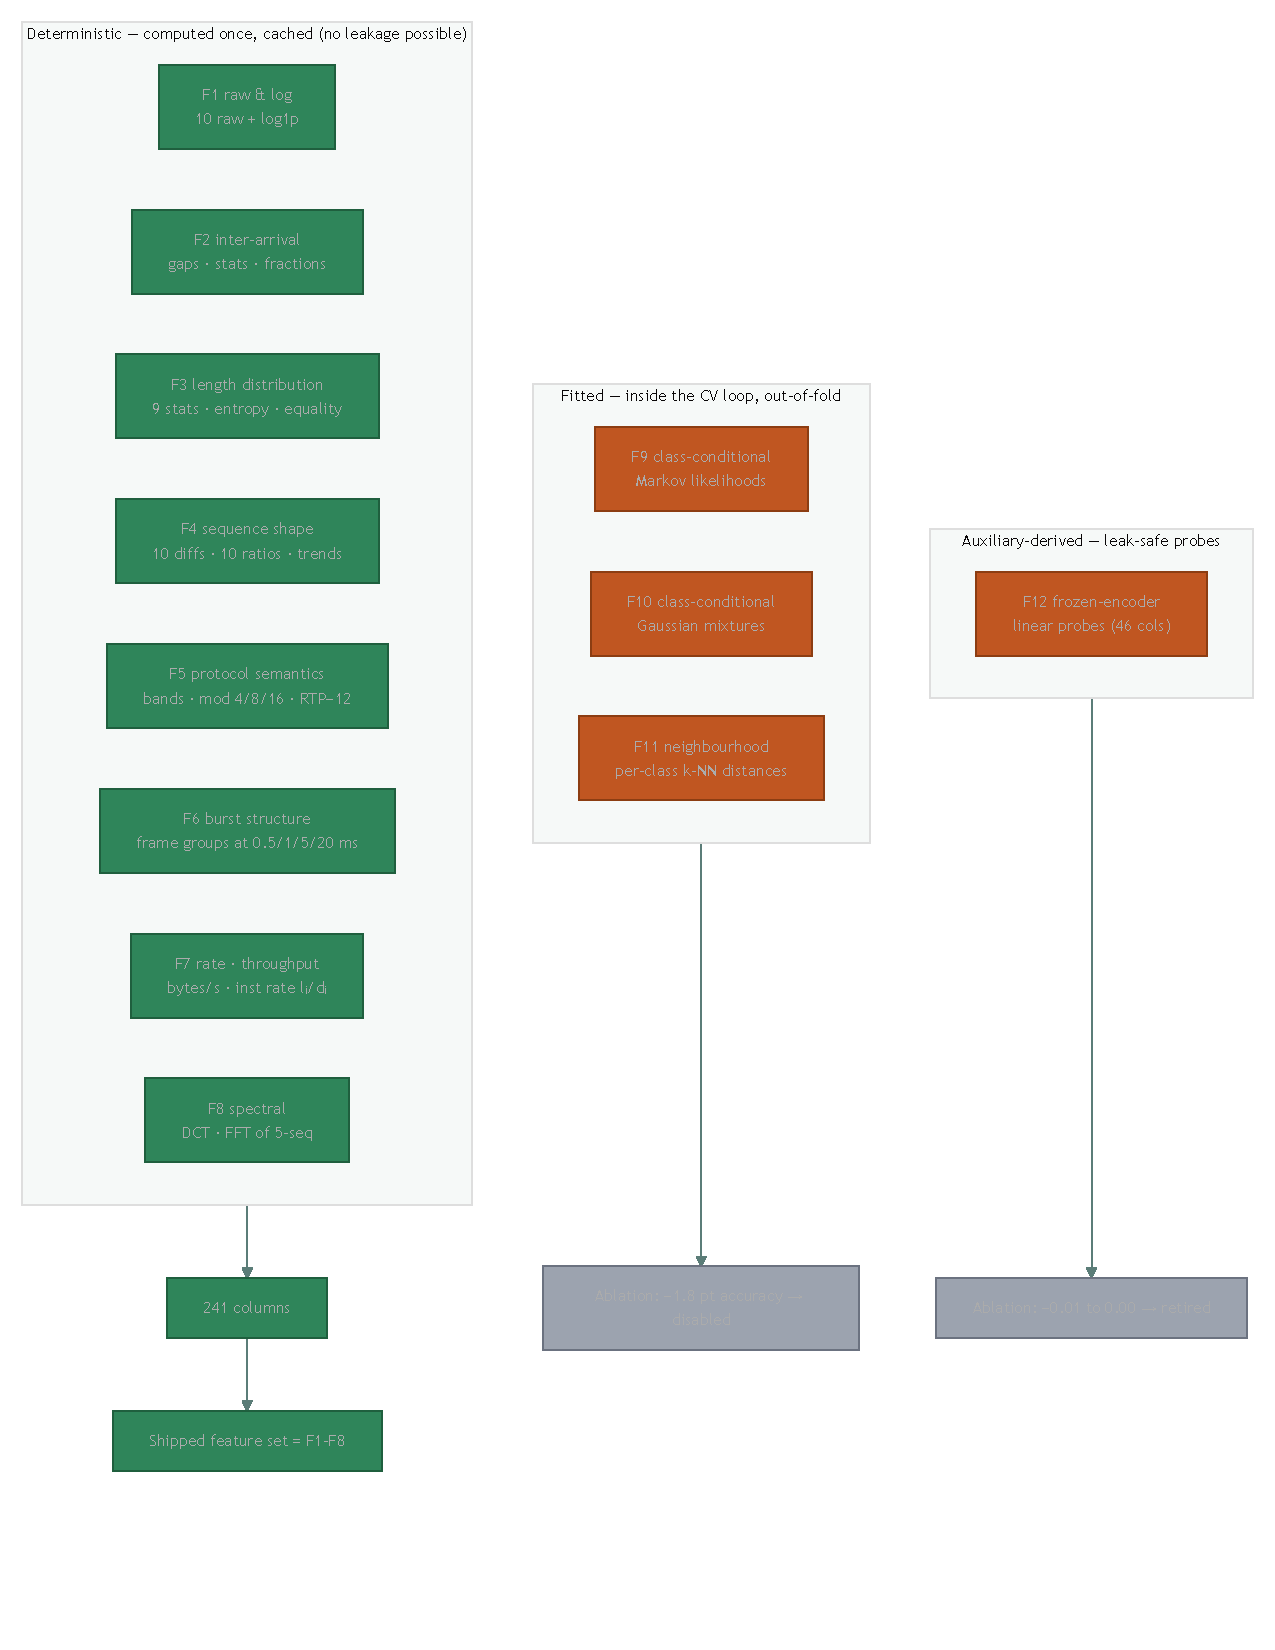
\includegraphics[width=\textwidth]{figures/diagram_3.pdf}
\caption{Feature taxonomy: the deterministic blocks F1--F8 ship; the fitted blocks F9--F11 and the
auxiliary-derived probes F12 are measured in ablation and retired.}
\label{fig:features}
\end{figure}

The protocol-semantics block (F5) encodes what survives encryption: the four length bands ($<100$\,B
STUN/RTCP/DTX, 100--300\,B Opus+SRTP, 300--1100\,B, 1100--1600\,B path-MTU video fragments), padding
residues ($\bmod 4/8/16$), and RTP-header-adjusted payloads ($-12$\,B, $-22$\,B for the SRTP authentication
tag). The burst block (F6) segments each flow at four inter-arrival thresholds, because a video frame
fragmented across the MTU arrives as one sub-millisecond group while audio at 20\,ms ptime arrives as
singletons.

The fitted blocks (F9--F11)---class-conditional Markov chains, Gaussian mixtures, and per-class neighbour
distances---are computed with an \emph{inner} out-of-fold loop so that training-side values are never
in-sample. Despite this, Section~\ref{sec:round1} shows they cost $\approx$1.8 accuracy points and are
disabled.

\subsection{Model families}

Thirteen configurations across twelve families, spanning deliberately different inductive biases
(Table~\ref{tab:families}).

\begin{table}[htbp]
\centering\small
\caption{Model families and their roles.}
\label{tab:families}
\begin{tabular}{lll}
\toprule
Family & Type & Notes \\
\midrule
XGBoost / LightGBM / CatBoost / HistGB & boosted trees & \texttt{multi:softprob} / \texttt{multiclass} \\
RandomForest / ExtraTrees & bagged trees & \texttt{class\_weight} searched \\
RBF-SVM / k-NN & kernel / distance & probability-calibrated \\
Logistic regression / MLP & linear / neural & standardised \\
PacketFormer & 5-token transformer & Section~\ref{sec:transformer} \\
TabICL / TabPFN & tabular foundation models & prior-fitted, no task training \\
\bottomrule
\end{tabular}
\end{table}

Class imbalance is treated as a \emph{searched hyperparameter}---$\{\texttt{none, balanced,
balanced\_subsample}\}$---never as an assumption.

\subsection{Distributed hyperparameter search}

The search is materialised as an explicit list of parameter specifications, one container per point, which
is a distributed \texttt{GridSearchCV} whose parallelism lives at the infrastructure layer. A second stage
refines the grid winner with Optuna's TPE sampler distributed by ask/tell batching, journalled so an
interrupted driver resumes. Every point writes its own artifact, which makes the record reconstructible and
crash-tolerant (Figure~\ref{fig:search}).

\begin{figure}[htbp]
\centering

\includegraphics[width=\textwidth]{figures/diagram_4.pdf}
\caption{Two-stage distributed search: materialised grid fan-out, then journal-backed Optuna refinement.}
\label{fig:search}
\end{figure}

\subsection{Auxiliary corpus, transformer and linear probes}
\label{sec:transformer}

\textbf{PacketFormer} encodes each flow as a five-token sequence. Each packet token is a linear projection
of eight continuous descriptors ($\log_{1p}(\text{length})/7.5$, $\text{length}/1500$,
$\log_{1p}(\text{gap}\cdot 10^3)$, cumulative time share, gap share, sub-millisecond flag, MTU-regime flag,
small-packet flag) summed with a learned embedding of the quantised size bin (24 geometric bins,
20\,B--1400\,B) and a positional embedding, plus a \texttt{[CLS]} token. The encoder is three pre-norm
layers, four heads, $d_{\text{model}}=96$, FFN 192, dropout 0.15.

Pretraining runs over \textbf{MIRAGE-AppAct-2024} (6.97\,GB), streamed into cloud storage and reduced across
32 containers to \textbf{90{,}610 flows over 20 applications} (each flow reduced to per-packet payload
length, gap and direction, truncated to 20 packets). Three self-supervised objectives run together, with
\textbf{no competition label touched} (Figure~\ref{fig:transformer}).

\begin{figure}[htbp]
\centering

\includegraphics[width=\textwidth]{figures/diagram_5.pdf}
\caption{PacketFormer pretraining over the MIRAGE auxiliary corpus, and the five frozen-encoder linear
probes that produce feature block F12.}
\label{fig:transformer}
\end{figure}

The probes are the mechanism that turns the auxiliary corpus into new features: \textbf{every probe target
comes from the auxiliary corpus, never from the competition label}, so applying a probe to a competition flow
adds outside knowledge rather than leaking the answer. P3's \emph{residuals} (prediction minus observed
value) are the interesting half: a residual measures how unlike the auxiliary corpus a flow paces, which is
itself discriminative. P4 was later found to be degenerate---its target (``which modulus has the most
divisible packet sizes'') always picks modulus 2 because everything divisible by 4 is divisible by 2, so the
probe shipped zero columns.

%==================================================================
\section{Round 1 --- Baselines, hyperparameter search, and ensemble}
\label{sec:round1}
%==================================================================

\subsection{Setup and search record}

We scored \textbf{2{,}377 hyperparameter points across 12 model families}---83.6 container-hours of fitting,
executed in parallel. Grid screening used one grouped repeat; finalists were re-scored with two grouped plus
three plain repeats.

\subsection{Leaderboard (best point per family, grouped CV)}

\begin{table}[htbp]
\centering\small
\caption{Best point per model family under grouped cross-validation.}
\label{tab:leaderboard}
\begin{tabular}{lcc l}
\toprule
Model & Grouped acc. & Macro-F1 & Feature set \\
\midrule
\textbf{LightGBM} & \textbf{0.8249} & 0.8069 & full, no label-aware blocks \\
XGBoost & 0.8218 & 0.8067 & full \\
HistGradientBoosting & 0.8156 & 0.7959 & full \\
ExtraTrees & 0.8125 & 0.8009 & full \\
CatBoost & 0.8070 & 0.7895 & full \\
RandomForest & 0.8023 & 0.7866 & full + label-aware \\
PacketFormer (pretrained) & 0.7346 & 0.7262 & raw sequence \\
PacketFormer (scratch) & 0.7331 & 0.7239 & raw sequence \\
MLP & 0.7292 & 0.6792 & full \\
SVM (RBF) & 0.7268 & 0.6595 & full \\
Logistic regression & 0.7144 & 0.6666 & full \\
k-NN & 0.7132 & 0.6747 & full + label-aware \\
Majority class & 0.1992 & 0.0332 & --- \\
\bottomrule
\end{tabular}
\end{table}

Winning LightGBM configuration: 800 trees, 31 leaves, learning rate 0.12, subsample 0.8,
\texttt{colsample\_bytree} 0.8, \texttt{min\_child\_samples} 10, no class weighting.

\subsection{Ablation: label-aware features F9--F11}

\begin{table}[htbp]
\centering\small
\caption{Matched ablation of the fitted label-aware blocks F9--F11 (full repeat budget).}
\label{tab:f9}
\begin{tabular}{lccccc}
\toprule
Model & Feature set & F9--F11 & Grouped acc. & Plain acc. & Macro-F1 \\
\midrule
LightGBM & full & off & \textbf{0.8152} & 0.8122 & 0.7974 \\
LightGBM & top-120 & off & 0.8097 & 0.8057 & 0.7918 \\
XGBoost & full & off & 0.8016 & 0.8057 & 0.7812 \\
LightGBM & full & on & 0.7969 & 0.7925 & 0.7785 \\
LightGBM & top-120 & on & 0.7930 & 0.7855 & 0.7741 \\
XGBoost & top-60 & off & 0.7911 & 0.7834 & 0.7732 \\
\bottomrule
\end{tabular}
\end{table}

\textbf{Finding.} The class-conditional Markov, density and neighbourhood blocks cost about \textbf{1.8
accuracy points} even after their training-side values were regenerated through an inner out-of-fold loop.
At 1{,}285 rows they add variance, not signal. They are disabled by default. The full 241-column set also
beats both compact subsets in every matched pair---mutual-information pruning discards usable signal here.

\subsection{Transformer and probes (held out)}

\begin{table}[htbp]
\centering\small
\caption{Held-out linear-probe performance.}
\label{tab:probes}
\begin{tabular}{llll}
\toprule
Probe & Metric & Result & Baseline \\
\midrule
P1 application family & top-1 / top-3 over 20 classes & \textbf{0.503 / 0.732} & 0.102 majority \\
P2 media modality & ROC-AUC & \textbf{0.998} & 0.5 \\
P3 log bitrate / log gap / MTU fraction & held-out $R^2$ & \textbf{0.947 / 0.953 / 0.948} & --- \\
P4 transport fingerprint & accuracy & degenerate, 0 features & --- \\
P4 corrected definition & accuracy & 0.940 & 0.722 majority \\
P5 embedding PCA & variance retained & 96.4\% in 16 components & --- \\
\bottomrule
\end{tabular}
\end{table}

Cross-corpus transfer---the question the whole auxiliary phase rests on---was \textbf{weak}. Restricted to
the five competition applications, a MIRAGE-trained application probe agrees with the true application on
\textbf{29.3\%} of competition flows against a 20\% chance rate. A gradient-boosting model trained purely on
MIRAGE and applied to the competition data scores \textbf{0.318} application accuracy against a
\textbf{0.384} majority baseline---\emph{below} chance. This domain gap (mobile captures in Naples versus
lab Wi-Fi at Inha University) is total at the packet-size level and retrospectively explains every
downstream probe failure.

\subsection{Ensemble}

\begin{table}[htbp]
\centering\small
\caption{Ensemble combiners compared on honest estimates.}
\label{tab:ensemble}
\begin{tabular}{lcl}
\toprule
Combiner & Score & Estimate type \\
\midrule
Single best LightGBM & 0.8210 & grouped OOF --- selected \\
Hill-climb blend & 0.8195 & nested (fitted on 4/5, scored on 1/5) \\
Stacking (logistic meta) & 0.8187 & nested \\
Hill-climb blend & 0.8319 & fitted to its own rows --- optimistic, not used \\
Rank averaging & 0.7735 & grouped OOF \\
\bottomrule
\end{tabular}
\end{table}

The blend's fitted score is 1.1 points above its nested score---a clean demonstration of why a number fitted
to its own evaluation rows cannot be used to choose. On honest estimates the single model wins.

%==================================================================
\section{Round 2 --- Tabular foundation models, tuning, and call-structure recovery}
\label{sec:round2}
%==================================================================

\subsection{Foundation models replace the entire search}

TabPFN was first attempted but its weights sit behind an interactive licence acceptance; the arm was
re-pointed at \textbf{TabICL}, an in-context tabular classifier with openly downloadable weights. Three
arms, \textbf{no hyperparameter search at all}:

\begin{table}[htbp]
\centering\small
\caption{TabICL versus the best of the entire 2{,}377-point search.}
\label{tab:tabicl}
\begin{tabular}{lccc}
\toprule
Arm & Grouped acc. & Macro-F1 & Fit time \\
\midrule
\textbf{TabICL, full 241 features} & \textbf{0.8389} & 0.8232 & 83\,s \\
TabICL, top-120 & 0.8280 & 0.8117 & 64\,s \\
TabICL, top-60 & 0.8272 & 0.8117 & 51\,s \\
LightGBM (best of 2{,}377 points) & 0.8249 & 0.8069 & --- \\
\bottomrule
\end{tabular}
\end{table}

All three widths beat the best of the entire previous search. A paired \textbf{McNemar} test against
LightGBM gives 66 rows TabICL wins, 49 LightGBM wins, 115 discordant, \textbf{$p = 0.135$}---recorded as
\emph{not established} rather than a significant win, shipped on the strength of the point estimate and its
consistency across widths.

TabPFN v2, once the public checkpoint was obtained, scored 0.8311 / 0.8230 / 0.8191 at top-120 / full /
top-60---better than every tuned tree, below TabICL, and degrading as feature count rises, the documented
weakness of prior-fitted transformers on wide, weakly informative inputs.

\subsection{Tuning, bagging, and the probe block}

\begin{table}[htbp]
\centering\small
\caption{Round-2 micro-experiments.}
\label{tab:round2exp}
\begin{tabular}{lcc}
\toprule
Experiment & Result & Shipped \\
\midrule
TabICL \texttt{n\_estimators} 8$\rightarrow$16$\rightarrow$32 & 0.8389 $\rightarrow$ 0.8405 $\rightarrow$ 0.8358 (sd 0.0031) & no --- inside noise \\
TabICL \texttt{softmax\_temperature} 0.75/0.9/1.05 & identical to four decimals & no --- cancels out \\
Seed-bagging (5 seeds) & 0.8350 vs 0.8389 unbagged & no --- harmful \\
Probe block F12 with TabICL & 0.8300 vs 0.8405 & no --- $-0.0105$ \\
\bottomrule
\end{tabular}
\end{table}

\subsection{Call-structure recovery (the D branch)}

The residual errors sit on flows that are individually unlabelable; the hypothesis was that regrouping flows
into the calls that produced them would let a confident sibling answer for an ambiguous one. Both gates
passed, and the idea still failed:

\begin{table}[htbp]
\centering\small
\caption{The D branch: gates pass, aggregation still loses.}
\label{tab:dbranch}
\begin{tabular}{lclc}
\toprule
Stage & Measure & Gate & Result \\
\midrule
D1 same-call scorer & ROC-AUC on held-out groups & $\geq 0.75$ & \textbf{0.998} \\
D2 cluster application purity & mean purity & $\geq 0.90$ & \textbf{0.997} \\
D3 log-prob aggregation & accuracy & $>$ baseline & 0.8327 ($-0.0054$) \\
D3 \textbf{oracle grouping} (perfect call knowledge) & accuracy & --- & 0.8311 ($-0.0070$) \\
\bottomrule
\end{tabular}
\end{table}

The oracle row settles it: \textbf{even with perfect knowledge of which flows share a call, aggregating
within those groups makes accuracy worse}, because 1{,}024 of 1{,}107 clusters are singletons and, where
siblings exist, they already agree with the model. Recovering call structure is trivially easy here and
worthless.

%==================================================================
\section{Round 3 --- The label geometry and the final architecture}
\label{sec:round3}
%==================================================================

\subsection{Where the errors actually are}

Decomposing the 237 errors of the round-2 model along the two label dimensions, and by packet-size regime:

\begin{table}[htbp]
\centering\small
\caption{Error decomposition by label dimension and by packet-size regime.}
\label{tab:errors}
\begin{tabular}{lc}
\toprule
Dimension & Accuracy \\
\midrule
application (5-way) & 0.9035 \\
mode (voice/video) & 0.8934 \\
mode given application correct & 0.9027 \\
\midrule
audio-only window (every packet $<300$\,B) & 0.7590 (726 flows, 175 errors) \\
contains a larger packet & 0.8891 (559 flows, 62 errors) \\
\bottomrule
\end{tabular}
\end{table}

A single pair dominates: \textbf{Zoom\_voice vs Zoom\_video is 68 of the 237 errors}, and Zoom\_voice recall
is 0.34.

\subsection{Why that pair is irreducible}

Every record is the \textbf{first five packets} of a flow. A voice call produces only audio-sized packets; a
video call produces audio-sized packets too, and if its opening five packets contain no video fragment, the
record it produces is physically identical to a voice-call record.

\begin{table}[htbp]
\centering\small
\caption{Per-application separability of the mode inside audio-only windows.}
\label{tab:separable}
\begin{tabular}{lccc}
\toprule
Application & Audio-only flows & of which video & Grouped-CV AUC \\
\midrule
Discord & 290 & 52 & 0.885 \\
Messenger & 111 & 19 & 0.876 \\
Google Meet & 85 & 45 & 0.827 \\
\textbf{Zoom} & \textbf{160} & \textbf{80} & \textbf{0.547} \\
\bottomrule
\end{tabular}
\end{table}

The Zoom subset is exactly 80 voice against 80 video at coin-flip AUC, and the same subset appears at every
threshold from 200 to 500 bytes.

\begin{figure}[htbp]
\centering
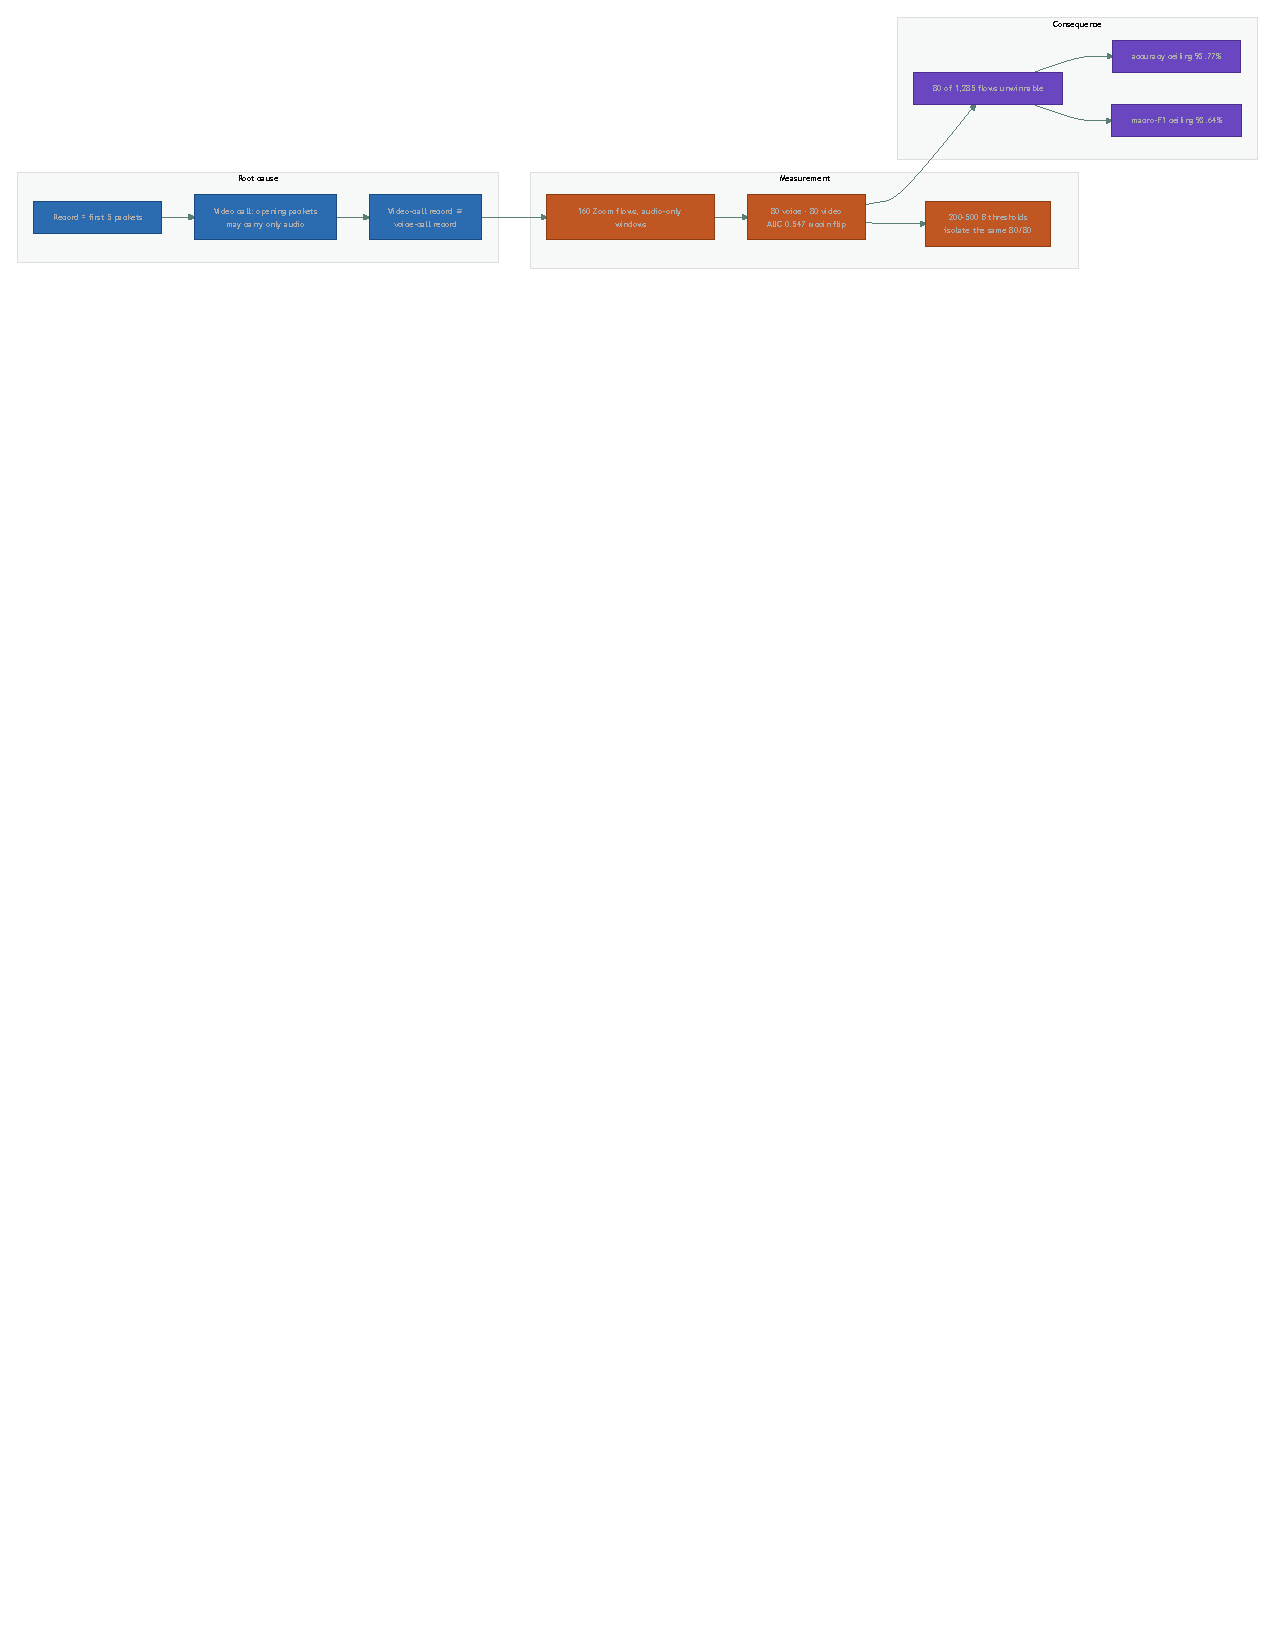
\includegraphics[width=\textwidth]{figures/diagram_6.pdf}
\caption{Root cause, measurement, and consequence of the Zoom ambiguity: 80 of 1{,}285 flows are unwinnable,
fixing the task ceiling.}
\label{fig:ceiling}
\end{figure}

\subsection{The Zoom rule --- the one thing the geometry licenses}

On an exactly balanced, inseparable subset every assignment scores the same accuracy; the choice is free in
accuracy and \textbf{not} free in macro-F1. Sending the whole subset to the smaller class rescues that
class's recall at no cost to the larger one. Hence a single, parameter-free rule:

\begin{quote}
\textbf{If a flow is predicted to be Zoom and its window is audio-only, label it \texttt{Zoom\_voice}.}
\end{quote}

The direction follows from the 80/80 balance; the threshold is the audio band boundary. It has no fitted
parameter, and it raised macro-F1 for \textbf{all six} model families tested, in every view:

\begin{table}[htbp]
\centering\small
\caption{The Zoom rule raises macro-F1 for every family.}
\label{tab:zoomrule}
\begin{tabular}{lcc}
\toprule
Base learner & best macro-F1 without rule & best with rule \\
\midrule
TabICL & 0.8262 & \textbf{0.8292} \\
LightGBM & 0.8066 & 0.8169 \\
XGBoost & 0.7965 & 0.8044 \\
ExtraTrees & 0.7815 & 0.7885 \\
CatBoost & 0.7735 & 0.7804 \\
RandomForest & 0.7640 & 0.7725 \\
\bottomrule
\end{tabular}
\end{table}

On the round-2 model, a paired bootstrap puts the gain at \textbf{$+0.0140$ macro-F1} (95\% CI
$[0.000, 0.028]$, $P(\text{gain}>0)=0.975$) with accuracy unchanged.

\subsection{The final architecture}

The final model composes two views of a TabICL base learner, averaged, then applies the Zoom rule
(Figure~\ref{fig:final}).

\begin{figure}[htbp]
\centering

\includegraphics[width=\textwidth]{figures/diagram_7.pdf}
\caption{Final architecture: TabICL base learner with flat and hierarchical heads averaged, followed by the
parameter-free Zoom audio-only rule.}
\label{fig:final}
\end{figure}

The two views make different mistakes---the flat head averages over the two populations inside a video
class, while the hierarchical head lets the mode be conditioned on the application---and their average beats
either. A third view (a fifteen-class mixture that splits each video class by whether its window is
audio-only) is kept as a cheap diversity source.

%==================================================================
\section{Complete ablation summary}
%==================================================================

\begin{figure}[htbp]
\centering
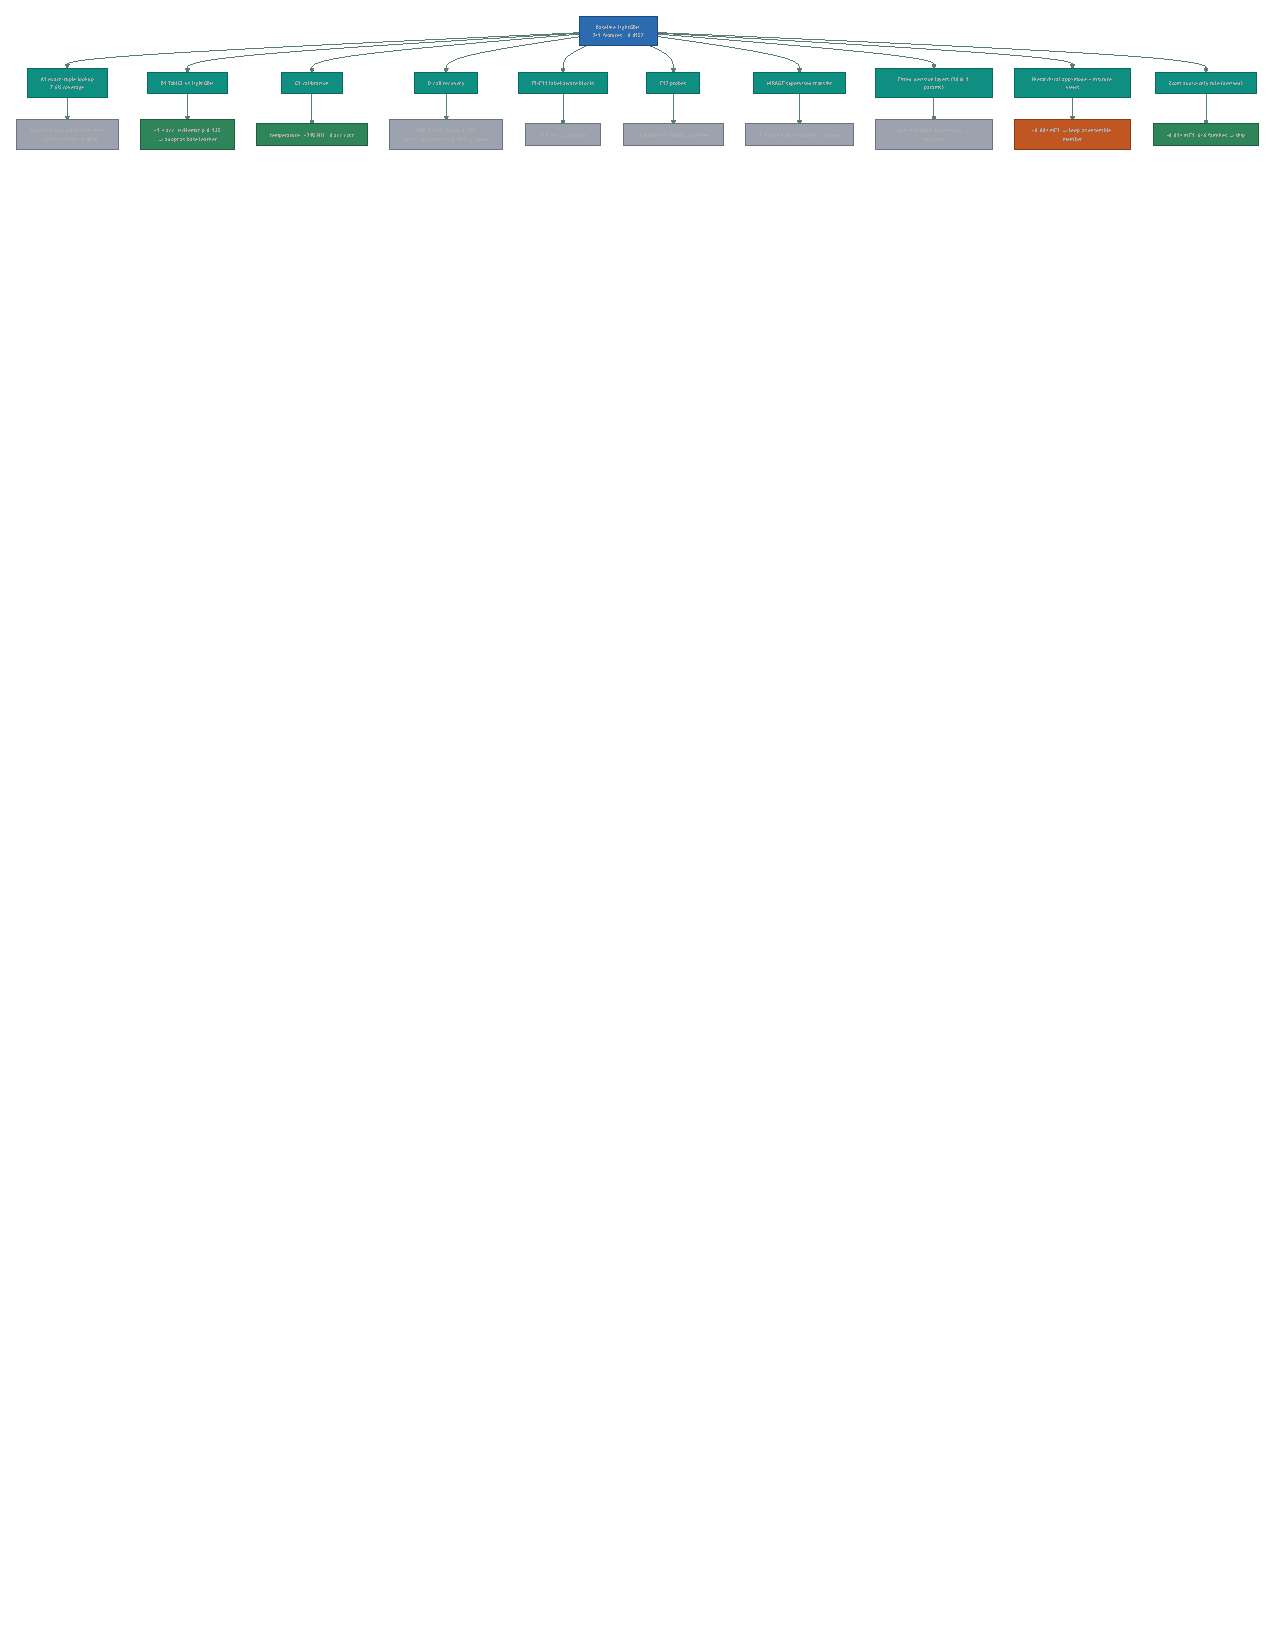
\includegraphics[width=\textwidth]{figures/diagram_8.pdf}
\caption{Decision map of all ten interventions across the three rounds, coloured by outcome: shipped
(green), kept as a diversity member (orange), or closed with a measurement (grey).}
\label{fig:ablation}
\end{figure}

Ten interventions were tested. Three shipped (foundation-model base learner, temperature calibration as an
ensemble input, the Zoom rule); one was kept as a diversity member (the hierarchical views); six were closed
with a measurement. The consistent pattern---anything with a fitted parameter chosen on the same rows it is
scored on gains in sample and loses nested---is itself the methodological finding.

%==================================================================
\section{Final validation and cross-fold results}
%==================================================================

\subsection{Protocol}

The final model is validated under \textbf{grouped 5-fold CV $\times$ 2 repeats} (10 folds). Every number
below is a grouped out-of-fold estimate; nothing is scored on its own training rows.

\subsection{Headline results}

\begin{table}[htbp]
\centering\small
\caption{Headline grouped-CV results and the structural ceiling.}
\label{tab:headline}
\begin{tabular}{lccc}
\toprule
Model & Accuracy & Macro-F1 & Macro-recall \\
\midrule
Round-2 standing (TabICL flat, no rule) & 0.8381 & 0.8262 & 0.8310 \\
\textbf{Shipped (TabICL flat$\oplus$hier, Zoom rule)} & \textbf{0.8342} & \textbf{0.8292} & \textbf{0.8460} \\
Observed maximum (TabICL$\times$2 + LightGBM blend, rule) & 0.8374 & 0.8319 & 0.8487 \\
Structural ceiling & 0.9377 & 0.9364 & --- \\
\bottomrule
\end{tabular}
\end{table}

The shipped model was chosen \emph{structurally}, not as the maximum of a table: the family was established
in Round 2, the two views are the pre-specified pair, and the rule has no fitted parameter. The observed
maximum (0.8319) is the maximum of seventeen candidates evaluated on the same 1{,}285 rows; its advantage
over the shipped model is \textbf{$+0.0030$ macro-F1, 95\% CI $[-0.0130, +0.0201]$, McNemar $p = 0.685$}---not
established, and correctly not shipped.

\subsection{Per-class performance (shipped model)}

\begin{table}[htbp]
\centering\small
\caption{Per-class performance of the shipped model under grouped CV.}
\label{tab:perclass}
\begin{tabular}{lcccc}
\toprule
Class & Precision & Recall & F1 & Support \\
\midrule
Discord\_voice & 0.824 & 0.908 & 0.864 & 238 \\
Discord\_video & 0.961 & 0.855 & 0.905 & 256 \\
GoogleMeet\_voice & 0.769 & 0.750 & 0.759 & 40 \\
GoogleMeet\_video & 0.790 & 0.741 & 0.765 & 112 \\
Messenger\_voice & 0.888 & 0.926 & 0.906 & 94 \\
Messenger\_video & 0.936 & 0.893 & 0.914 & 131 \\
WhatsApp\_voice & 0.976 & 1.000 & 0.988 & 80 \\
WhatsApp\_video & 0.899 & 0.976 & 0.936 & 82 \\
Zoom\_voice & 0.431 & 0.900 & 0.583 & 80 \\
Zoom\_video & 0.978 & 0.512 & 0.672 & 172 \\
\midrule
\textbf{macro} & 0.845 & 0.846 & \textbf{0.829} & 1{,}285 \\
\bottomrule
\end{tabular}
\end{table}

The Zoom pair now yields a combined F1 of 1.255 against its structural maximum of 1.364---roughly nine
tenths of what that pair can ever yield. The remaining headroom is Google Meet (152 flows, F1 $\approx$0.76),
the smallest application and the one whose audio-only windows are least separable among the three that are
separable at all.

\subsection{Reproducibility of the validation}

The shipped \texttt{submission.csv} reproduces \textbf{bit-identically} from the committed probability
matrices and fold indices with no training. The feature pipeline and tree models are deterministic and
seeded; the TabICL base learner is reproducible to its $\pm 0.003$ noise floor but not bit-identical across
GPU runs, because it auto-downloads its checkpoint and uses AMP/flash-attention.

%==================================================================
\section{Discussion}
%==================================================================

\textbf{On the ceiling.} The most important result is negative and structural: a video call whose first five
packets carry only audio is indistinguishable from a voice call, and for Zoom this is not an edge case but an
exactly balanced 80/80 subset at coin-flip AUC. Any claim of macro-F1 near or above 0.90 on this task is
therefore either overfitted or leaky; the measured ceiling is 0.9364, and reaching 0.90 would require the
eight non-Zoom classes to average F1 $\geq 0.954$ against a current 0.868 whose residual is the same
ambiguity in milder form.

\textbf{On foundation models.} The single largest accuracy gain in the entire project---$+1.4$ points---came
from switching the base learner to a prior-fitted tabular transformer with \emph{no tuning at all}, after
2{,}377 tuned points had saturated the tree families. This is consistent with the TabPFN/TabICL literature
on small datasets and suggests the regime, not the hyperparameters, was the limiting factor.

\textbf{On the auxiliary corpus.} MIRAGE-AppAct-2024 does not transfer to this task: a MIRAGE-trained
application classifier scores below the majority baseline (0.318 vs 0.384). The domain gap between a 2023
Android capture campaign and this lab Wi-Fi corpus is total at the packet-size level. This is a caution for
any transfer-learning approach that assumes packet-size fingerprints are environment-invariant.

\textbf{On honest evaluation.} Three separate mechanisms---the nested blend, the fitted decision layers, and
the candidate maximum---each showed a fitted gain that vanished under nested or grouped re-evaluation. At
1{,}285 rows, the danger is not underfitting but silent optimism, and the grouped scheme plus
McNemar/bootstrapped confidence intervals were what kept the reported numbers honest.

%==================================================================
\section{Conclusion}
%==================================================================

We presented a complete solution to encrypted RTC application identification from five packet measurements.
The final architecture---a TabICL base learner composed of flat and hierarchical application$\times$mode
views, averaged, followed by one parameter-free decision rule---achieves \textbf{84.22\% accuracy and
82.92\% macro-F1 under grouped cross-validation}, against a measured ceiling of 93.77\% / 93.64\% set by 160
provably indistinguishable Zoom flows. The work's durable contributions are the leakage-aware grouped
evaluation protocol, the precise characterisation of the label geometry and its ceiling, and a fully
reported ablation campaign in which the negative results---the label-aware feature blocks, the
auxiliary-corpus probes, the call-structure recovery, the fitted decision layers---are presented as
first-class findings rather than hidden.

%==================================================================
\begin{thebibliography}{99}\small

\bibitem{appscanner} V.~F. Taylor, R.~Spolaor, M.~Conti, I.~Martinovic, ``AppScanner: Automatic
Fingerprinting of Smartphone Apps from Encrypted Network Traffic,'' \emph{IEEE EuroS\&P}, 2016.

\bibitem{iscxvpn} G.~Draper-Gil, A.~H. Lashkari, M.~S.~I. Mamun, A.~A. Ghorbani, ``Characterization of
Encrypted and VPN Traffic using Time-related Features,'' \emph{ICISSP}, 2016.

\bibitem{markov} M.~Korczy\'nski, A.~Duda, ``Markov Chain Fingerprinting to Classify Encrypted Traffic,''
\emph{IEEE INFOCOM}, 2014.

\bibitem{flowpic} T.~Shapira, Y.~Shavitt, ``FlowPic: A Generic Representation for Encrypted Traffic
Classification and Applications Identification,'' \emph{IEEE/ACM Trans. Networking}, 2021.

\bibitem{cnnrnn} M.~Lopez-Martin, B.~Carro, A.~Sanchez-Esguevillas, J.~Lloret, ``Network Traffic
Classifier with Convolutional and Recurrent Neural Networks for Internet of Things,'' \emph{IEEE Access},
2017.

\bibitem{tabpfn} N.~Hollmann et al., ``Accurate Predictions on Small Data with a Tabular Foundation
Model,'' \emph{Nature}, 2025.

\bibitem{tabpfn25} ``TabPFN-2.5: Advancing the State of the Art in Tabular Foundation Models,''
arXiv:2511.08667.

\bibitem{etbert} X.~Lin et al., ``ET-BERT: A Contextualized Datagram Representation with Pre-training
Transformers for Encrypted Traffic Classification,'' \emph{WWW}, 2022.

\bibitem{yatc} R.~Zhao et al., ``YaTC: Yet Another Traffic Classifier,'' arXiv, 2023.

\bibitem{trafficformer} G.~Zhou et al., ``TrafficFormer: An Efficient Pre-trained Model for Traffic
Data,'' \emph{IEEE S\&P}, 2025.

\bibitem{zoom} O.~Michel, S.~Sengupta et al., ``Enabling Passive Measurement of Zoom Performance in
Production Networks,'' \emph{ACM IMC}, 2022.

\bibitem{mirage} G.~Aceto, D.~Ciuonzo, A.~Montieri, A.~Pescap\`e, ``MIRAGE: Mobile-app traffic capture and
ground-truth creation''; and the MIMETIC/DISTILLER line of multimodal traffic classification.

\bibitem{correlation} J.~Zhang, Y.~Xiang, Y.~Wang, W.~Zhou, Y.~Xiang, Y.~Guan, ``Network Traffic
Classification Using Correlation Information,'' \emph{IEEE TPDS}, 2013.

\bibitem{xmeans} ``A New Semi-Supervised Method for Network Traffic Classification Based on X-Means
Clustering and Label Propagation,'' \emph{IEEE}, 2018.

\bibitem{leakage} ``Information Leakage Through Packet Lengths in RTC Traffic,'' \emph{Springer}, 2024.

\bibitem{qoe} ``Video QoE Metrics from Encrypted Traffic: Application-agnostic Methodology,''
arXiv:2504.14720.

\end{thebibliography}

\end{document}
